\begin{figure}[htb]
  \centering
  \caption{Transition Maps (No Migration)}
  \begin{minipage}[t]{0.4\textwidth}
    \centering
    \small{(a) $\Delta$ Mean Welfare (CE)}
    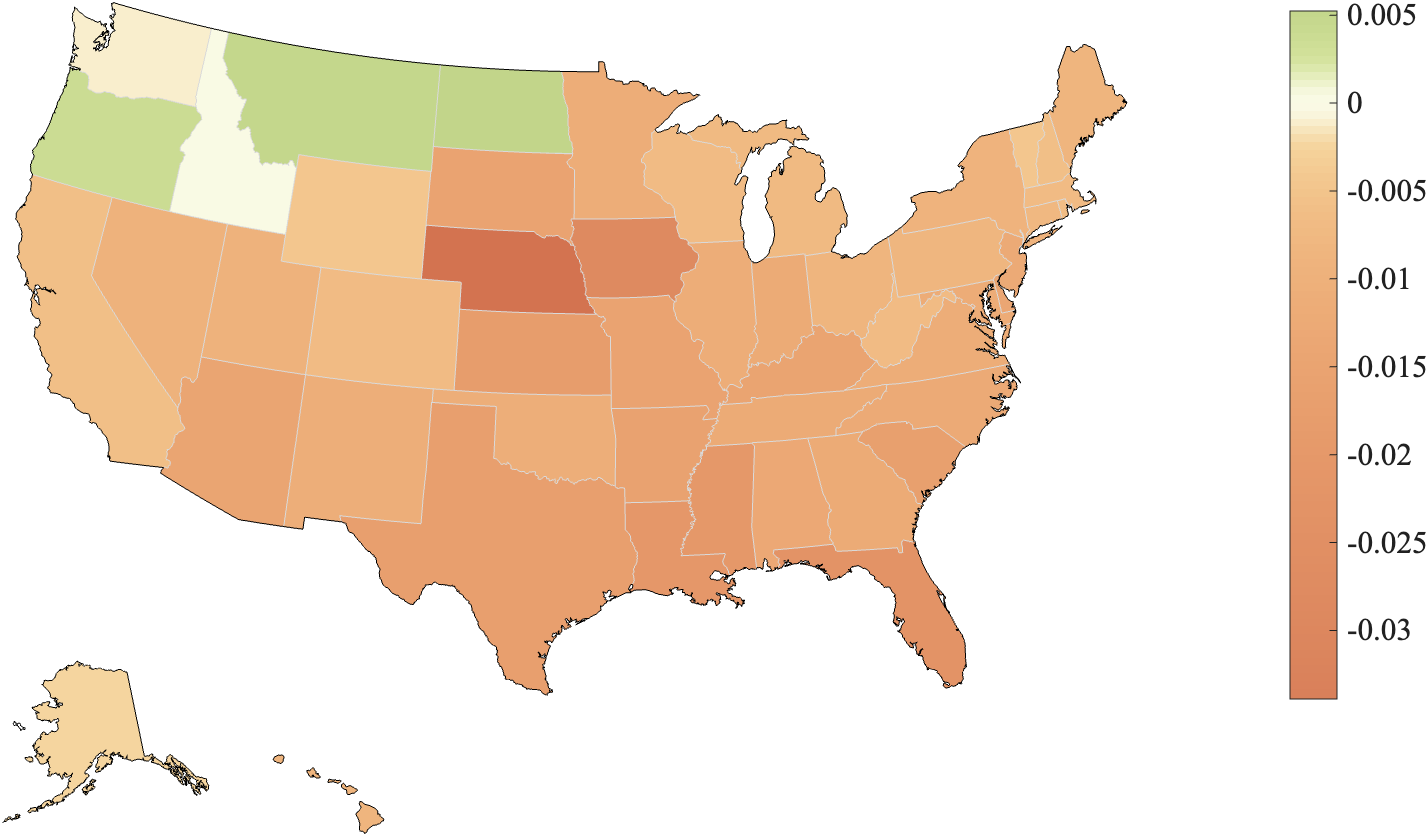
\includegraphics[width=\textwidth]{../Output/big_nu/graph_no_migration_did/transition_maps/transition_maps_delta_mean_welfare_ce.png}
  \end{minipage}\hfill
  \begin{minipage}[t]{0.4\textwidth}
    \centering
    \small{(b) $\Delta$ W/Y Ratio in level}
    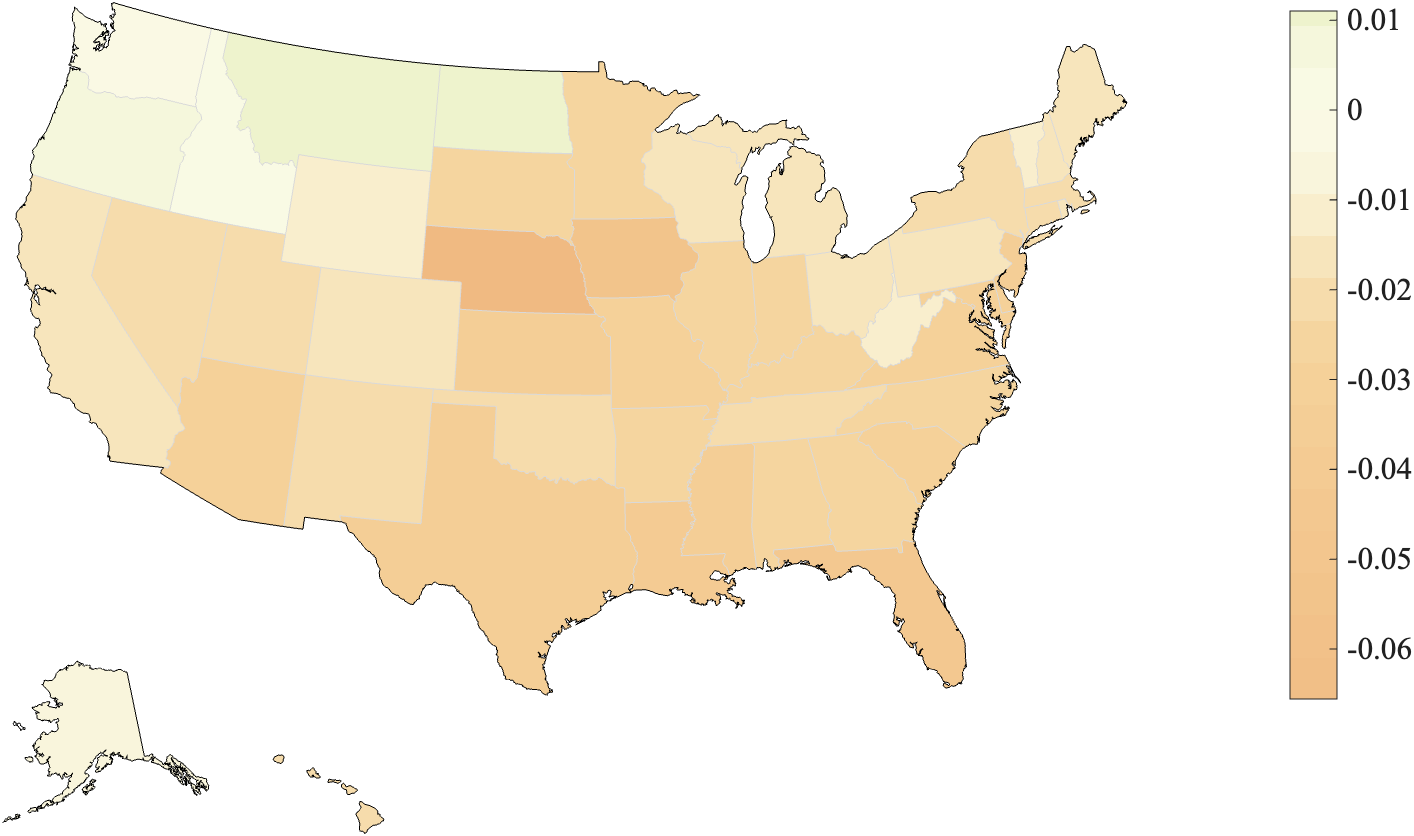
\includegraphics[width=\textwidth]{../Output/big_nu/graph_no_migration_did/transition_maps/transition_maps_wealth_income_ratio_changes.png}
  \end{minipage}
  \vspace{1em}
  \begin{minipage}[t]{0.4\textwidth}
    \centering
    \small{(c) $\Delta$ Local Population (\%)}
    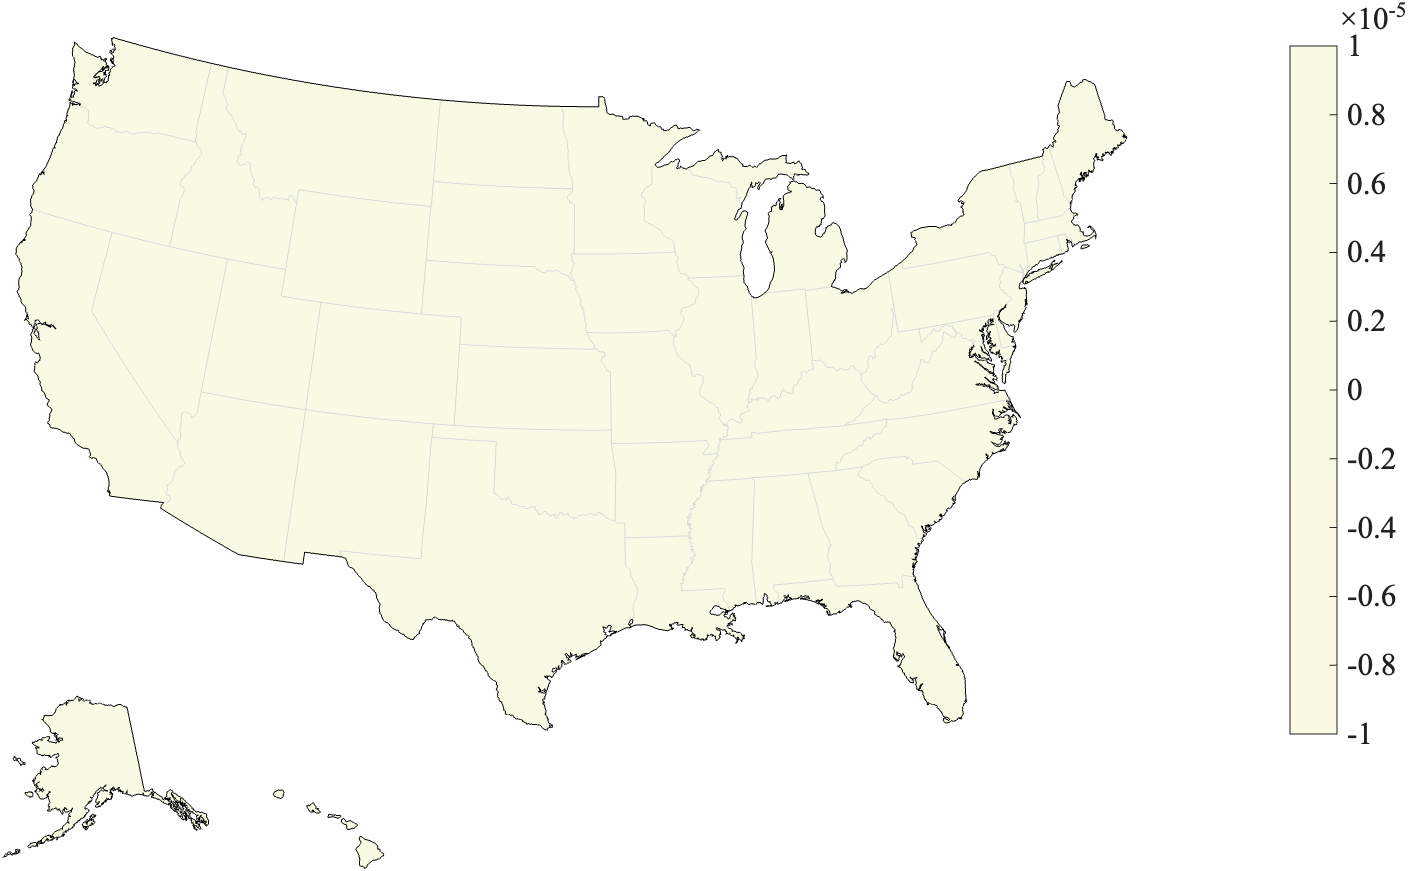
\includegraphics[width=\textwidth]{../Output/big_nu/graph_no_migration_did/transition_maps/transition_maps_local_pop_changes_pct.png}
  \end{minipage}\hfill
  \begin{minipage}[t]{0.4\textwidth}
    \centering
    \small{(d) $\Delta$ Mean Wealth (\%)}
    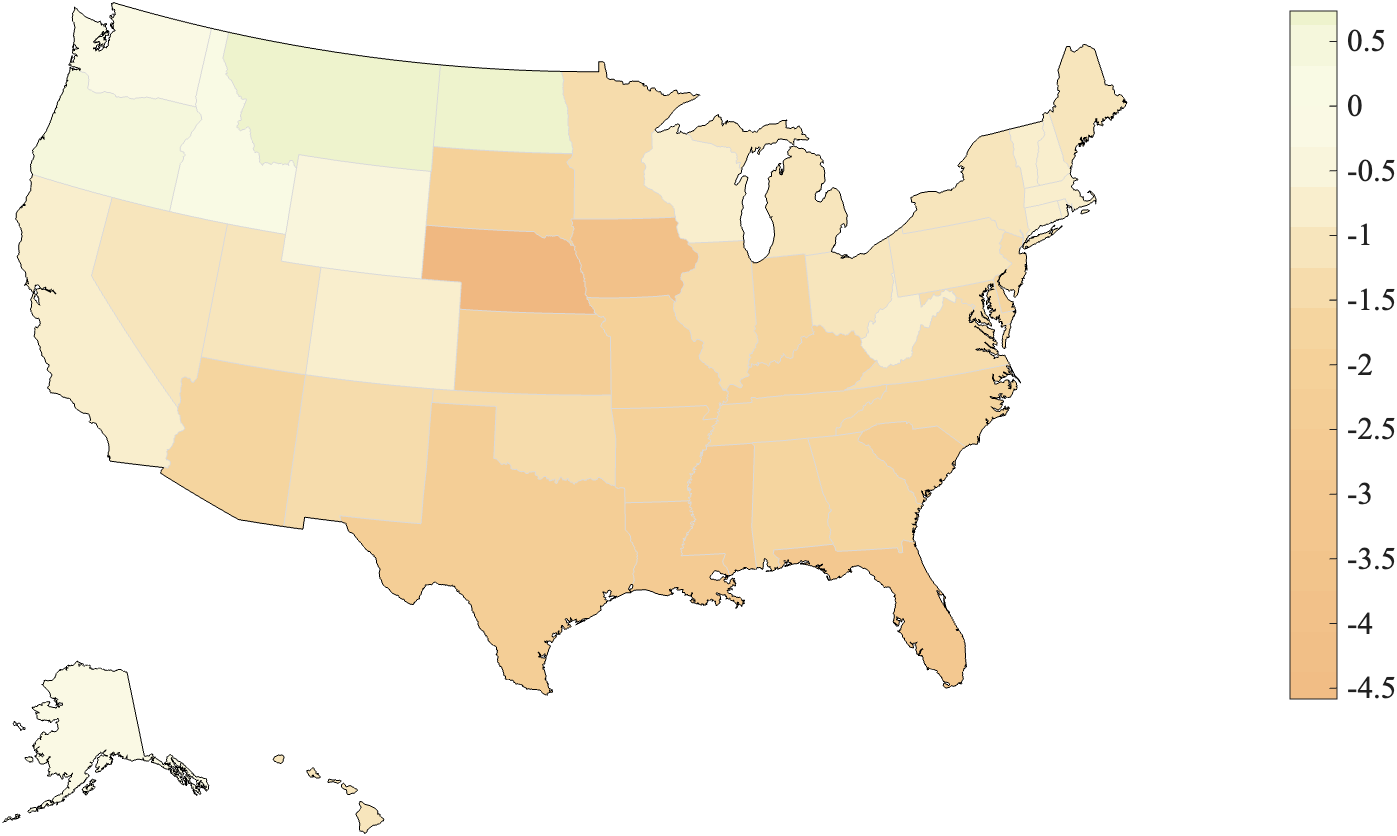
\includegraphics[width=\textwidth]{../Output/big_nu/graph_no_migration_did/transition_maps/transition_maps_pop_changes_pp.png}
  \end{minipage}
  \begin{minipage}{\textwidth}
  \vspace{0.5em}
  \footnotesize{\textbf{Note:} Spatial maps comparing the terminal steady state under 2100 climate parameters ($SS_\text{term}$) to the initial 2010 baseline steady state ($SS_\text{init}$) under No Migration autarky. Panel (a): change in mean Certainty Equivalent welfare $\Delta \text{CE}_\ell = \overline{\text{CE}}_{\ell, \text{term}} - \overline{\text{CE}}_{\ell, \text{init}}$. Panel (b): change in state wealth-to-earnings ratio $\Delta (W/Y)_\ell = (W/Y)_{\ell, \text{term}} - (W/Y)_{\ell, \text{init}}$. Panel (c): relative population change $\Delta L_\ell\% \equiv 0$. Panel (d): percentage change in state mean per-capita wealth $\Delta \bar{a}_\ell\%$.} \end{minipage}
  \label{fig:spatial_hetero_no_migration}
\end{figure}